\vspace*{\fill}
\section*{Infusing deep neural networks with physics}
\label{sec:lolaintro}
\begin{centering}
\textit{
The previous chapter ended by mentioning two ingredients that will become important for future searches with the multi-dimensional fit: A better vector boson tagger, and a generic anti-QCD tagger for signal independent searches. As a side project during my final PhD semester, I worked on a solution for the first, which has the added benefit of being a stepping stone towards the latter. This is what I will cover in the final chapter of this thesis.
\newline
\newline
When applying machine learning to particle physics problems, the input has historically consisted of pre-computed high-level features (quantities based on lower-level variables and certain theoretical assumptions).
With the rise of deep learning however, computational graphs have achieved an increased capability to find even the smallest correlations in datasets, allowing them to construct complex features on their own. The deep neural network (DNN) I will present in the following is based on the assumption that, given sufficient instructions about the laws of Nature, a neural network should be capable of reconstructing its own high-level features based on lower-level variables only. In addition, if smartly designed, the network should be capable of finding novel correlations and physical features, a-priori unknown, by allocating a physical meaning to the training weights deep within the network. The deep neural network I will present here, is trained to discriminate quark/gluon jets from W-jets. However, as I will discuss in the final section of this chapter, it is also the perfect starting point for developing a generic anti-QCD tagger.
\newline
\newline
The work presented in the following has not been published and still qualifies as work in progress. However, I believe developing taggers such as these is of great importance for future versions of the searches presented here, and is something I hope to continue working on in the future..
}
\begin{figure}[b!] 
    \centering
    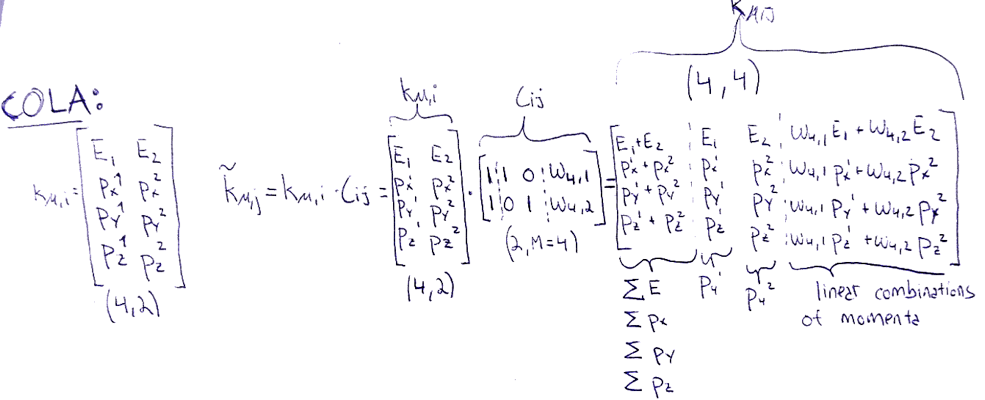
\includegraphics[width=7cm]{figures/vtagging/misc/cola.png}
    \vspace*{5mm}
    \caption*{\footnotesize{\textit{ ``What can we teach the machine?'' $\rightarrow$``What can we learn from the machine?''.\newline Work in progress}}}
\end{figure}
\end{centering}
\clearpage
\section{LoLa}
LoLa is a deep neural network architecture which was first introduced for top tagging~\cite{Butter:2017cot}. It is based on the idea that, given enough information about the laws of Nature, a neural network should be capable of calculating jet substructure observables on its own given only low-level information. The network is designed to discriminate between AK R=0.8 jets originating from W bosons from those originating from quarks or gluons, solely based on the jet constituent four-vectors (variables with little discriminating power on their own) as illustrated in Figure~\ref{fig:lola:4vec}.
\begin{figure}[h!]
\centering
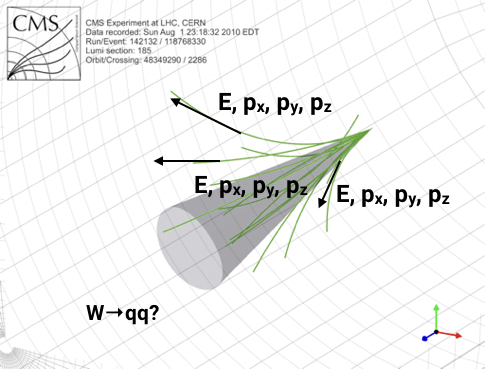
\includegraphics[width=0.33\textwidth]{figures/vtagging/misc/4vec.png}
\caption{LoLa uses only jet constituent four-vectors as input to discriminate W from q/g jets.}
\label{fig:lola:4vec}
\end{figure}
Rather than being fed high-level features, the neural network is given tools to perform calculations on Lorentz vectors using the Minkowski metric. Through two novel layers, linear combinations similar to jet clustering and jet substructure algorithms are performed, allowing the algorithm to create its own substructure variables. Additionally, training weights deep within the network correspond to physical quantities reconstructed by the algorithm; distance between particles, masses and energies, linear combinations of particle four-vectors etc.
Besides the end goal of discriminating Ws from quarks and gluons, one could therefore hope to learn of new correlations separating QCD from vector boson jets.

\subsection{Architecture}
The LoLa architecture is designed as a four layer deep, feed-forward sequential network doing supervised learning on fixed size input vectors.
Two novel layers are introduced, the Combination Layer (CoLa) and the Lorentz Layer (LoLa), which perform basic jet clustering and substructure calculations as well as implements the Minkowski metric.
These two layers are then followed by two fully connected layers, consisting of 100 and 50 nodes respectively, before the final output is computed using a Softmax activation function, yielding two output probabilities between 0 and 1. The loss function to be minimized is "categorical crossentropy" (or log loss) where the two categories in use are W versus non-W probabilities. Only the W jet probability is stored.
The optimizer used in the training is the, now standard, ADAM optimizer~\cite{DBLP:journals/corr/KingmaB14}, which adapts the learning rate of the model parameters during training. The code itself is written using the Keras~\cite{chollet2015keras} interface with a TensorFlow~\cite{tensorflow2015-whitepaper} backend.
The full architecture with input and output dimension per layer is shown in Figure~\ref{fig:lola:arch}. The three first boxes are matrices, while the final four boxes correspond to vectors of different length. In the following, each layer will be explained in detail.
\begin{figure}[h!]
\centering
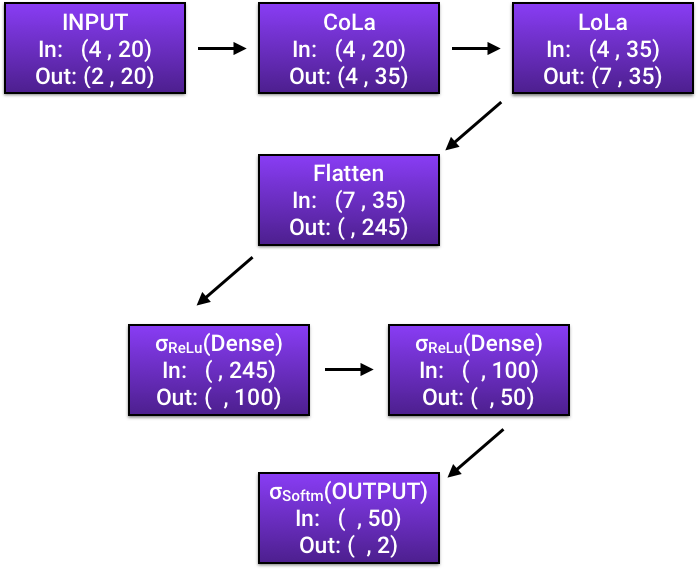
\includegraphics[width=0.59\textwidth]{figures/vtagging/misc/architecture.png}
\caption{The full LoLa architecture. ``In'' denotes the dimension of the input tensor to the given layer, ``Out'' is the output tensors dimensions.}
\label{fig:lola:arch}
\end{figure}


\subsection{Input}
This algorithm is trained to discriminate between fully merged hadronic W-jets coming from the process $\BulkG \rightarrow WW \rightarrow q\bar{q}q\bar{q}$ (where $M_{\BulkG}=0.6-4.5\TeV$), and quark/gluon jets from a QCD sample generated with \PYTHIA{8}Pythia 8. All jets are clustered with the anti-\kt algorithm with a distance parameter of R=0.8, with the PUPPI pileup removal algorithm applied. In addition, they are required to have $\PT > 200 \GeV$ and $|\eta| < 2.5$. 
Jets are defined as W-jets if they are matched to a generator level hadronically decaying W bosons, with the following matching criteria:
The generated vector boson needs to be within $\Delta R < 0.6$ of the jet axis, and the quark decay products need to be within $\Delta R < 0.8$ of the jet axis. The \PT and $\eta$ distribution of signal and background jets, is shown in Figure~\ref{fig:lola:kinematics}.
\begin{figure}[h!]
\centering
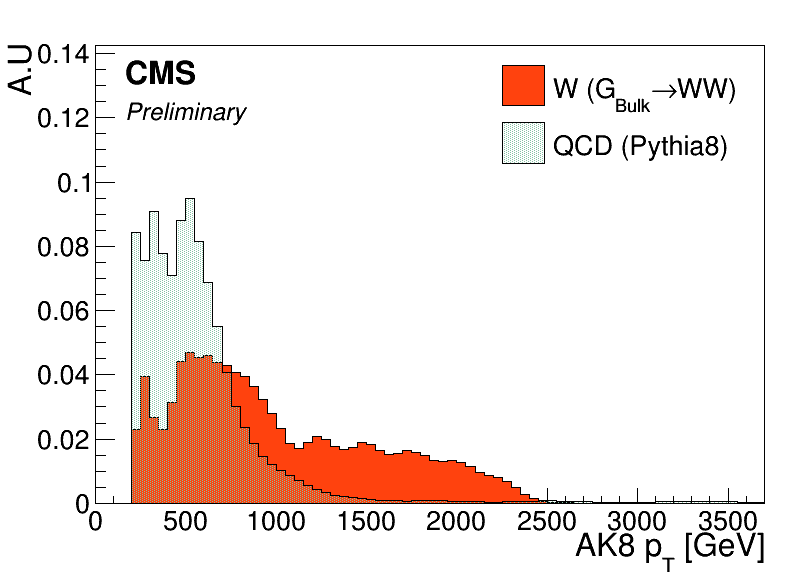
\includegraphics[width=0.4\textwidth]{figures/vtagging/AN-18-099/input/inputs/sig-bkg/jpt.png}
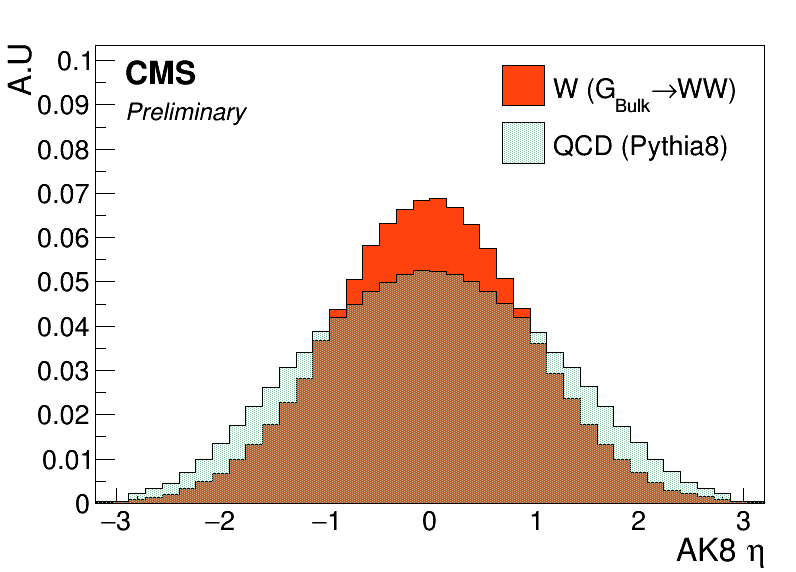
\includegraphics[width=0.4\textwidth]{figures/vtagging/AN-18-099/input/inputs/sig-bkg/jeta.png}\\
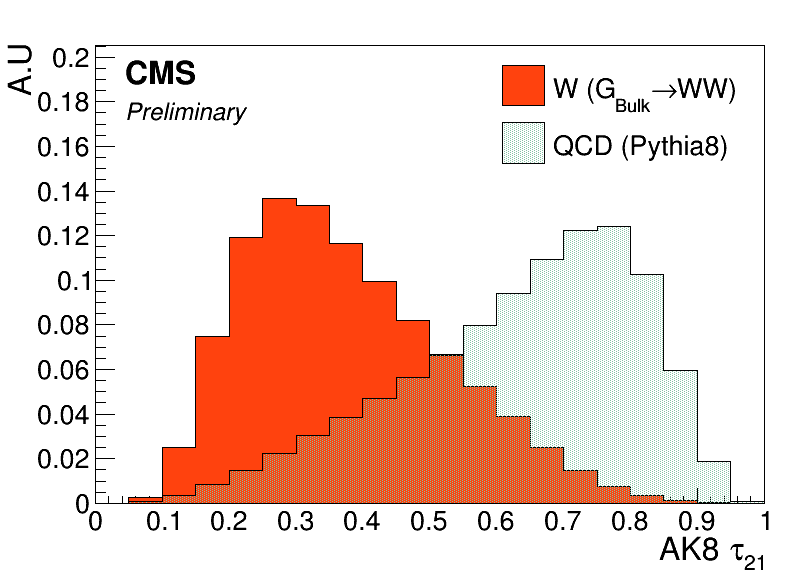
\includegraphics[width=0.4\textwidth]{figures/vtagging/AN-18-099/input/inputs/sig-bkg/jtau21.png}
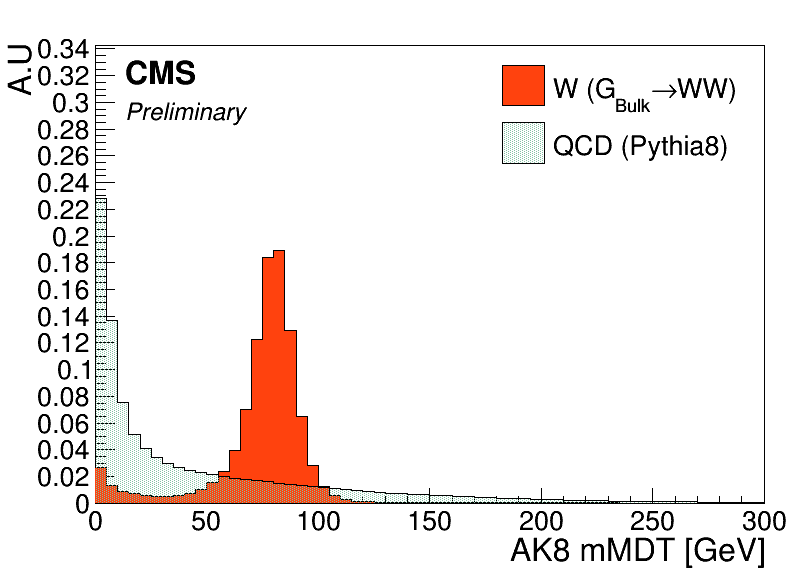
\includegraphics[width=0.4\textwidth]{figures/vtagging/AN-18-099/input/inputs/sig-bkg/msoftdrop_beta0.png}
\caption{Jet \PT (top left), $\eta$ (top right), \nsubj (bottom left) and softdrop jet mass (bottom right) for signal and background jets.}
\label{fig:lola:kinematics}
\end{figure}
From these signal and background jets, only the jet constituent four vectors of the 20 highest-\PT particles are used as input to the deep neural network: $E$, $p_x$, $p_y$ and $p_z$. I use 20 constituents as any larger number has a negligible affect on the performance, while performance tends to drop once going below 15. The input is therefore a $4 \times N=20$ matrix for each signal and background jet, one four-vector for each of the 20 jet constituents:
\begin{equation}
x_{\mu,i}=\begin{pmatrix}
E^1 & E^2 & \dots & E^N \\[1ex]
p_x^1 & p_x^2 & \dots & p_x^N \\[1ex]
p_y^1 & p_y^1 & \dots & p_y^N \\[1ex]
p_z^1 & p_z^2 & \dots & p_z^N
\end{pmatrix}
\end{equation}
The total number of jet constituents is shown in Figure~\ref{fig:lola:nconst}, and the input variables (here for all constituents) is shown in Figure~\ref{fig:lola:inputs}.\newline
\begin{figure}[h!]
\centering
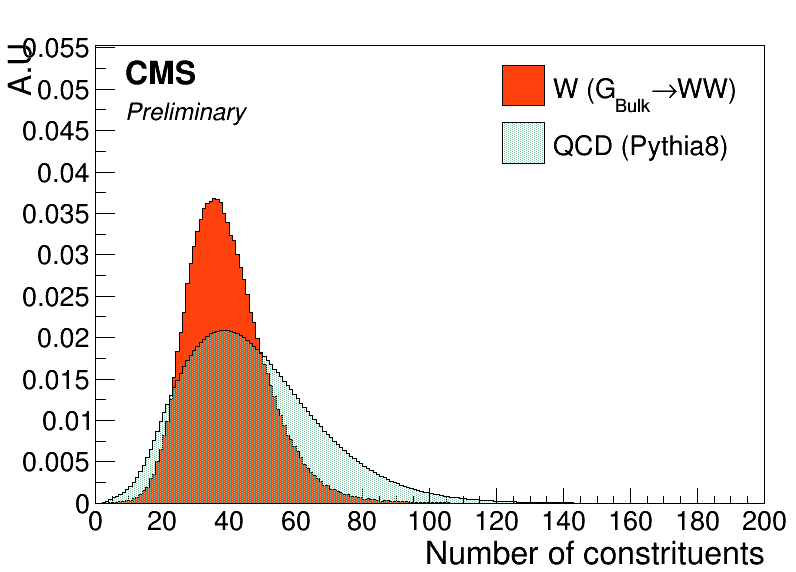
\includegraphics[width=0.4\textwidth]{figures/vtagging/AN-18-099/input/inputs/sig-bkg/nconst.png}
\caption{The number of jet constituents for signal (red) and background (blue). Only the 20 highest-\PT constituents are used during training.}
\label{fig:lola:nconst}
\end{figure}
\begin{figure}[h!]
\centering
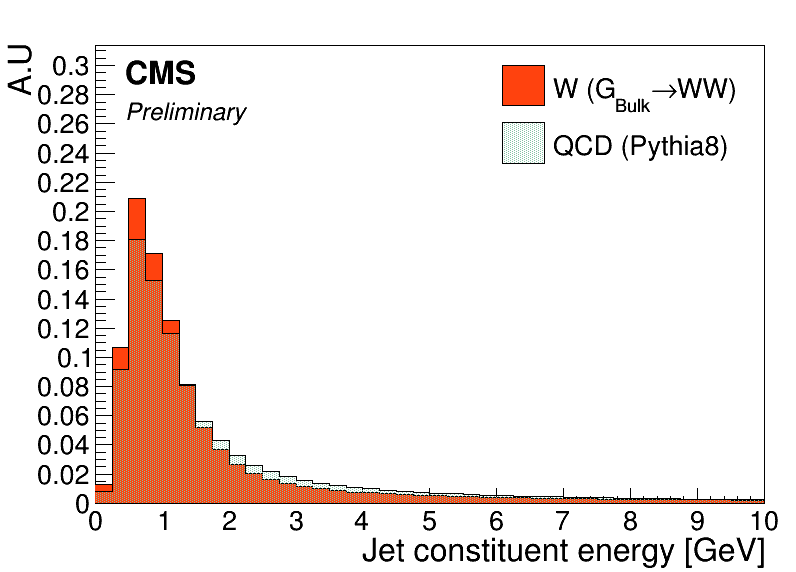
\includegraphics[width=0.4\textwidth]{figures/vtagging/AN-18-099/input/inputs/sig-bkg/pe.png}
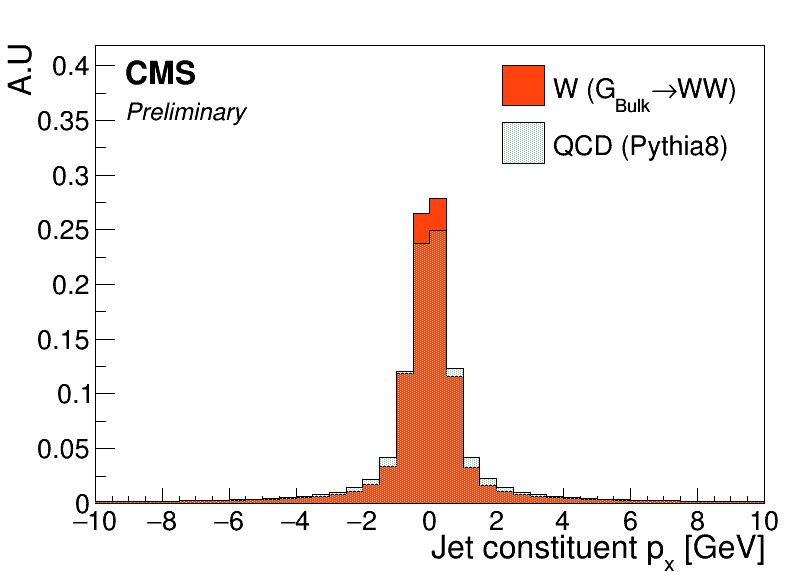
\includegraphics[width=0.4\textwidth]{figures/vtagging/AN-18-099/input/inputs/sig-bkg/ppx.png}\\
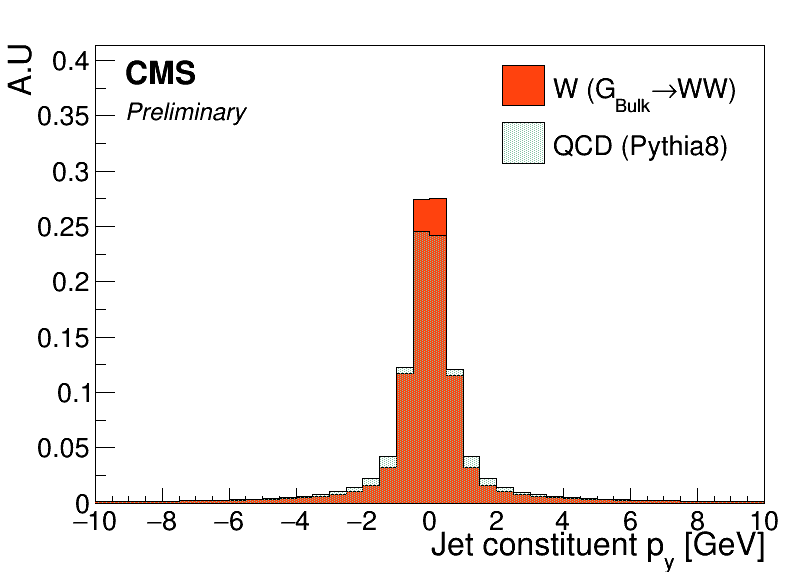
\includegraphics[width=0.4\textwidth]{figures/vtagging/AN-18-099/input/inputs/sig-bkg/ppy.png}
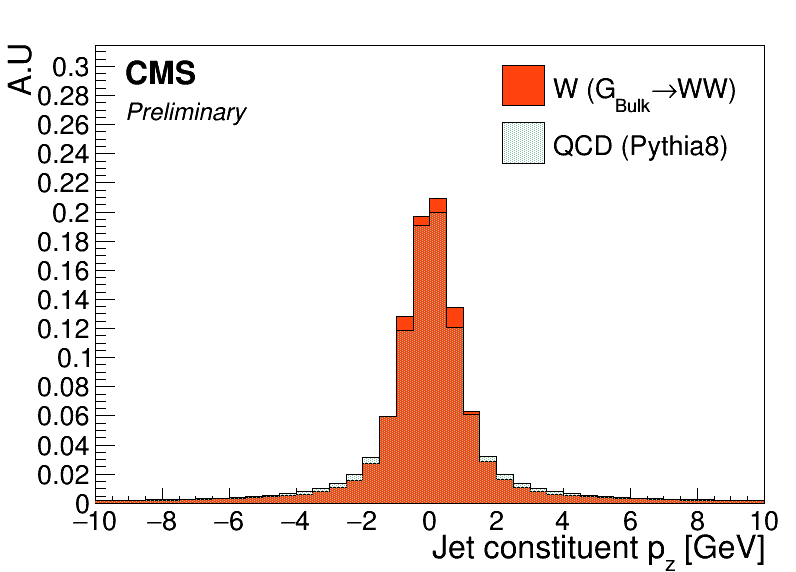
\includegraphics[width=0.4\textwidth]{figures/vtagging/AN-18-099/input/inputs/sig-bkg/ppz.png}
\caption{Energy (top left), $p_x$ (top right), $p_y$ (bottom left) and $p_z$ (bottom right) for all jet constituents. These values are used as input to the neural network training.}
\label{fig:lola:inputs}
\end{figure}
It is clear that the input variables provide little discriminating power on their own. Therefore, the network must learn how to derive other physical quantities where the signal and background PDFs differ to a larger extent. This is achieved through the two custom layers described in the following.

\subsection{The Combination Layer}
\label{sec:cola}
The Combination Layer (CoLa) consists of a matrix which, when takin the scalar product with the input matrix, compute linear combinations of the jet constituents, similar to what is done in recombination jet algorithms. The main goal here is to create additional four-vectors as input for the next layer. The CoLa matrix is a concatenation of the following: A vector of 1's of length $N$, the $N \times N$ identity matrix ($N=20$) and a matrix of $N \times M$ trainable weights.
\begin{equation}
  C_{i,j}=\begin{pmatrix}
1 & 1 & 0 & \dots & 0 & w_{1,N+2} & w_{1,N+3}                & \dots & w_{1,(N+2)+M)} \\
1 & 0 & 1 & \dots & 0 & w_{2,N+2} & w_{2,N+3}                & \dots & w_{2,(N+2)+M)} \\
\vdots & \vdots & \vdots & \ddots & \vdots & \vdots & \vdots & \vdots & \vdots \\
1 & 0 & 0 & 0 & 1 & w_{N,N+2} & w_{N,N+3}                    & \dots & w_{N,(N+2)+M)} 
\end{pmatrix}
\end{equation}
When performing the following multiplication
\begin{equation}
  x_{\mu,i}^{C} = x_{\mu,i}  C_{i,j}
\end{equation}
the resulting output matrix will have dimensions $4 \times (1+N+M)$ and consists of the following: A first column containing the sum of all constituent momenta, the four-momenta of each individual constituent, and M=14 different linear combinations of particles with trainable weights. The first corresponds to the neural network computing the four-vector of the ``full'' jet, at least the full jet in terms of its 20 highest-\PT constituents. The second, simply passes each original constituent four-momentum to the next layer. The final, and most interesting part, lets the network construct alternative subjet four-vectors by letting it weigh constituents up and down as it sees fit in order to reach optimal discrimination power. As an example, lets look at the effect of CoLa in the simple case of only two input jet constituents and two trainable linear combinations:
\begin{equation*}
  \footnotesize
  \begin{centering}
  \begin{pmatrix}
    E^1 & E^2\\[1ex]
    p_x^1 & p_x^2\\[1ex]
    p_y^1 & p_y^1\\[1ex]
    p_z^1 & p_z^2
  \end{pmatrix}
  \begin{pmatrix}
    1 & 1 & 0 & & w_{1,4} & w_{1,5}\\[1ex]
    1 & 0 & 1 & & w_{2,4} & w_{2,5}\\
  \end{pmatrix}
  = \begin{pmatrix}
    E^1  +E^2   & E^1   & E^2   & w_{1,4}E^1   + w_{2,4}E^2   & w_{1,5}E^1  +w_{2,5}E^2    \\[1ex]
    p_x^1+p_x^2 & p_x^1 & p_x^2 & w_{1,4}p_x^1 + w_{2,4}p_x^2 & w_{1,5}p_x^1+w_{2,5}p_x^2  \\[1ex]
    p_y^1+p_y^1 & p_y^1 & p_y^1 & w_{1,4}p_y^1 + w_{2,4}p_y^1 & w_{1,5}p_y^1+w_{2,5}p_y^1  \\[1ex]
    p_z^1+p_z^2 & p_z^1 & p_z^2 & w_{1,4}p_z^1 + w_{2,4}p_z^2 & w_{1,5}p_z^1+w_{2,5}p_z^2
  \end{pmatrix}
   \end{centering}
\end{equation*}
 In the two last columns, the neural network makes two ``subjet'' four-vectors by weighting the relative contribution of each particle as it sees fit. This is similar to jet grooming (Section~\ref{sec:objreco:grooming}) or PUPPI pileup subtraction (Section~\ref{subsub:objreco:puppi}), and should allow the network to learn which constituents are part of the hard scatter and which are not. The $x_{\mu,i}^{C}$ matrix is finally passed on to the next layer, the Lorentz Layer.
\subsection{The Lorentz Layer}
The Lorentz Layer (LoLa) is responsible for encoding how particles move in space-time through a simple set of rules. Each column (four-vector) of $x_{\mu,i}^{C}$, is used to compute, and afterwards is replaced by, the following $k=7$ features:
\begin{equation}
  \label{eq:lola:lola}
  x_{k,i}^{L} = \begin{pmatrix}
  m^2  (x_{\mu,i}^{C})                       \\[1ex]
  \PT  (x_{\mu,i}^{C})                       \\[1ex]
  w^E_{ij} E(x_{\mu,j}^{C})                       \\[1ex]
  w^{s1}_{ij}\sum d^2(x_{\mu,i}^{C},x_{\mu,j}^{C}) \\[1ex]
  w^{s2}_{ij}\sum d^2(x_{\mu,i}^{C},x_{\mu,j}^{C}) \\[1ex]
  w^{m1}_{ij}\min d^2(x_{\mu,i}^{C},x_{\mu,j}^{C}) \\[1ex]
  w^{m2}_{ij}\min d^2(x_{\mu,i}^{C},x_{\mu,j}^{C}) 
  \end{pmatrix}
\end{equation}
Going through from top to bottom, these are:
\begin{itemize}
  \item The invariant mass and \PT of each four-vector
  \item A linear combination of all four-vector energies where each is scaled by a trainable weight
  \item The sum of distances between the four-vector under consideration and every other column reweighted with a trainable weight
  \item The minimum distance between the four-vector under consideration and every other column where each distance again is reweighted by a trainable weight.
 \end{itemize}
  The Minkowski metric enters explicitly in the first and in the last four calculations, where the neural network is told to abide by the rules
\begin{equation}
  m^2 (x_{\mu,i}^{C}) = g^{\mu\nu}x_{\mu,i}^{C}x_{\nu,i}^{C}
\end{equation}
and
\begin{equation}
  d^2 (x_{\mu,i}^{C},x_{\mu,j}^{C}) = (x_{\mu,i}^{C}-x_{\mu,j}^{C})_{\mu} g^{\mu\nu} (x_{\mu,i}^{C}-x_{\mu,j}^{C})_{\nu}
\end{equation}
with $g^{\mu,\nu}=[-1,1,1,1]$, when calculating the invariant mass and distance between particles/subjets. This tells the neural network to use a space-time geometry in all its calculations to respect Lorentz Invariance. The four final rows of LoLa are the most interesting: Here the network computes quantities similar to n-subjettiness by summing up the distances between all constituents, the jet axis and the subjets produced by CoLa. If, for instance, the network has been capable of reconstructing two hard subjets in the final columns of CoLa, which do linear combinations of particles, it can create its own ``$\tau_2$'' variable by taking the distance between those subjets and all the jet constituents (and weighing down the column corresponding to the full jet four-vector, column one). Then it can do the same by calculating the distance between the full jet four-vector and all constituents (now weighing down the linear combinations) and compute``$\tau_2$''.\par

The two custom layers, CoLa and LoLa, therefore come together in order to encode jet clustering and substructure in a novel way. They provide the network with the necessary tools in order to create its own physical quantities, through linear combinations with trainable weights, which then again are used to produce other physical quantities with new trainable weights. This allows the network full freedom to explore all interesting particle correlations, where the resulting output features have a physical meaning that can be probed.\newline
LoLa turns the question ``What can we teach the machine?'' around to ``What can we learn from the machine?''. 

\section{Performance}
The deep neural network is trained on 320k signal and background jets for up to 100 epochs, but allow for an early stopping after ten epochs if the loss is stable. The test sample consists of 60k W jets and 60k quark/gluon jets.
To quantify the performance we look at the signal efficiency versus mistagging rate comparing the performance of LoLa to that of the taggers used previously in this thesis: PUPPI softdrop with \nsubj and PUPPI softdrop with \ddt.
The performance of these three different taggers, is shown in Figure~\ref{fig:lola:roc}. The point where the blue curves end, represent the signal efficiency for a mass cut of 65 \GeV $<$ Softdrop jet mass $< $105 \GeV, here roughly 70\%.
\begin{figure}[h!]
\centering
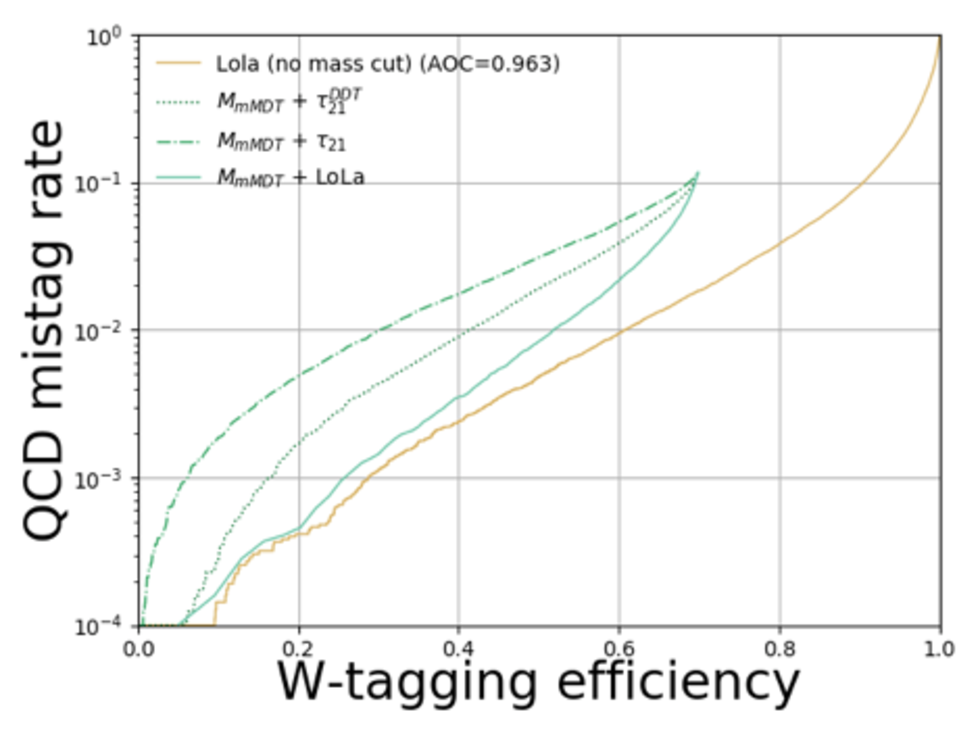
\includegraphics[width=0.4\textwidth]{figures/vtagging/AN-18-099/training/LoLa-comp-roc.pdf}
\caption{Performance of LoLa compared to other W-tagging discriminants in the background-signal efficiency plane: PUPPI softdrop + \nsubj (dashed blue), PUPPI softdrop + \ddt (dotted blue), LoLa with a softdrop mass window applied (solid blue) and the nominal LoLa tagger with no mass cut applied.}
\label{fig:lola:roc}
\end{figure}
We clearly see that LoLa performs significantly better than the current baseline W-taggers based on \nsubj and \ddt, with a roughly 20\% higher signal efficiency at a given mistagging rate. LoLa also has a higher signal acceptance, as it can be used without a mass window applied. If LoLa were to replace the tagger used in Search II (a better comparison than Search III as the latter uses a rather unconventional mass window), which has a signal efficiency of $\sim42\%$ at a $2\%$ mistagging rate for a single jet, the signal efficiency for the same mistagging rate would be 65\%, a 55\% increase. For an analysis requiring two tagged jets, that would imply going from an 18 to a 43\% total signal efficiency, a significant gain.

\section{Dependence on jet mass and \PT}
Despite being a key feature, absolute performance is not all that quantifies how good one tagger is compared to another. One a tagger is planned to be used in physics analysis, there are three key questions one needs to consider:
\begin{itemize}
    \itemsep0em 
    \item Is the absolute performance better (compared to common methods)?
    \item Is the tagger \PT-dependent?
    \item Does the tagger sculpt the mass spectrum?
\end{itemize}
These three measures are equally important in quantifying performance and, in the following, I will attempt to explain why this is the case and which approaches are used here in order to tackle them.\par
Any deep neural network trained to distinguish W jets from q/g jets, will naturally learn that \PT and mass are discriminating features unless it is penalized for it. Figure~\ref{fig:lola:corr} shows the LoLa discriminant as a function of jet \PT and softdrop jet mass. 
\begin{figure}[h!]
\centering
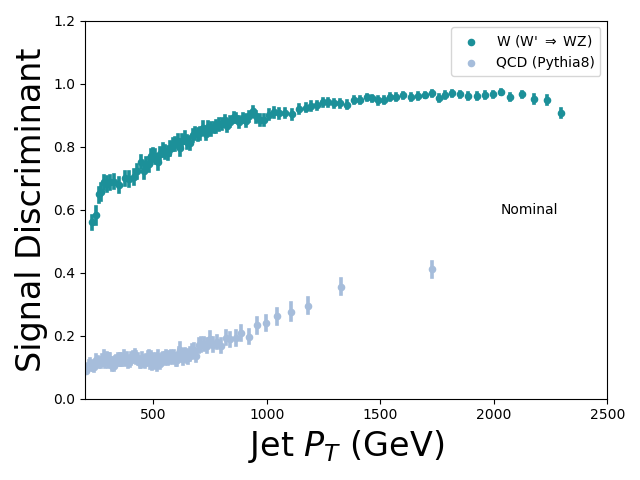
\includegraphics[width=0.4\textwidth]{figures/vtagging/lola/wLola_v6_500rew-profile-jpt.png}
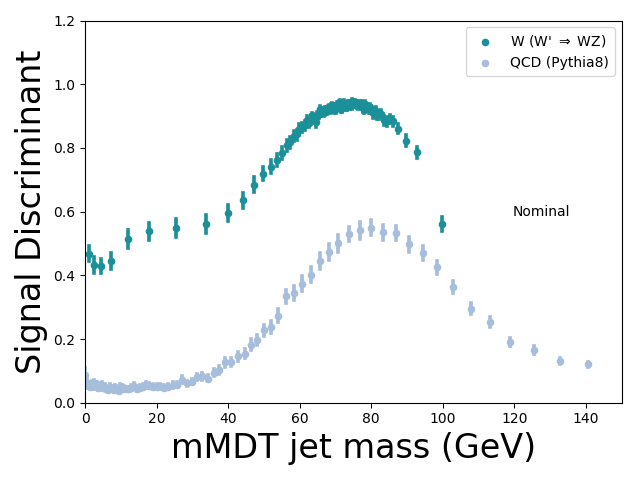
\includegraphics[width=0.4\textwidth]{figures/vtagging/lola/wLola_v6_500rew-profile-jsd0.png}
\caption{The LoLa discriminant as a function of jet \PT (left) and softdrop jet mass (right). A strong correlations with both variables is observed}
\label{fig:lola:corr}
\end{figure}
A strong correlation is observed both for signal and for background jets (closer to 1 means more signal like), with a rising slope as a function of \PT (meaning the network interprets a higher jet \PT as more signal like) and a bump around the W mass for both signal and for background.

\subsection{\PT-decorrelation}
A tagger which is \PT dependent is a problem for the following reasons: Firstly, the signal efficiency is variable, which requires a working point that scales with \PT. That in itself is not problematic and can easily be computed. However, it implies that when computing efficiency scale factors from data, a range of different scale factors for different working points is required. In addition, the performance is measured at low \PT, a region where the tagging efficiency can be substantially different from the analysis signal region due to the strong \PT correlation present. Finally, the dijet invariant mass is intrinsically linked to the \PT spectrum, meaning that any \PT dependence in addition can introduce sculpting of the dijet invariant mass spectrum.\newline
From the top left plot in Figure~\ref{fig:lola:kinematics}, one clearly sees that the jet \PT distribution is very different for signal and for background. In order to avoid that the network learns jet \PT to be a discriminating feature, I therefore compute a jet-by-jet weight intended to flatten the jet \PT spectrum. This weight is passed as a sample weight to the training set, reweighting each jets contribution to the total loss (making high mass QCD jets and low mass signal jets count more). Figure~\ref{fig:lola:ptweight} shows the jet \PT distribution without any \PT-reweighting applied (solid lines) and after applying a \PT-weight (dashed lines).
\begin{figure}[h!]
\centering
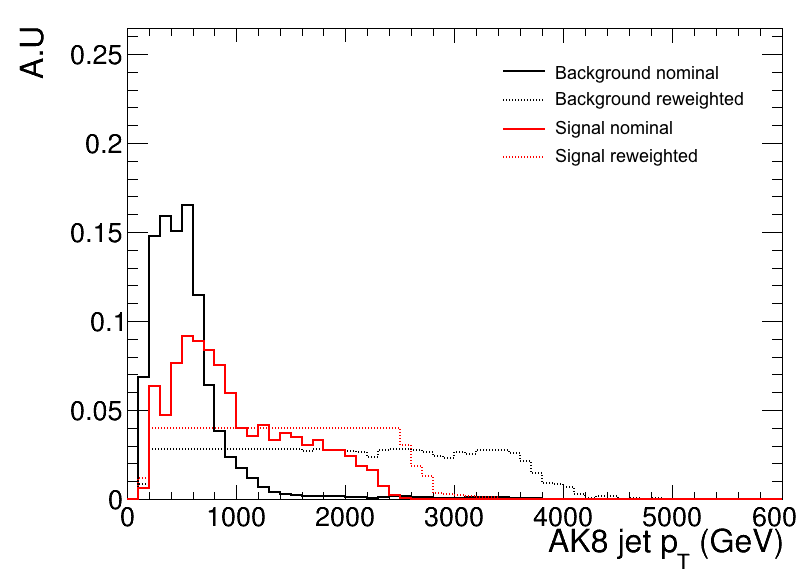
\includegraphics[width=0.4\textwidth]{figures/vtagging/AN-18-099/input/pt_reweighted/postWeight.png}
\caption{Jet \PT distribution before (solid lines) and after (dashed line) applying a weight intended to flatten the jet \PT spectrum.}
\label{fig:lola:ptweight}
\end{figure}
The training is then repeated, this time passing a sample weight with each jet, and the final discriminant compared to the nominal training. Figure~\ref{fig:lola:rocptweighted} shows the performance of the same taggers as above but with one additional line, LoLa \PT-reweighted.
\begin{figure}[h!]
\centering
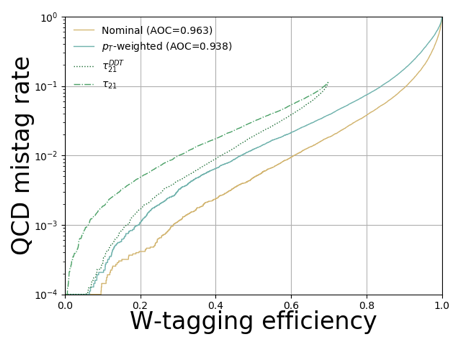
\includegraphics[width=0.4\textwidth]{figures/vtagging/AN-18-099/training/lolaptrew.png}
\caption{Performance of the \PT-reweighted LoLa tagger (solid blue) and the nominal LoLa tagger (solid yellow).}
\label{fig:lola:rocptweighted}
\end{figure}
A clear drop in performance is observed, as expected when removing information from the training. However, when we again look at the discriminant output as a function of jet \PT in Figure~\ref{fig:lola:ptweightedcorr}, the correlation we observed before has vanished and we are left with a tagger not depending on the jet \PT.
\begin{figure}[h!]
\centering
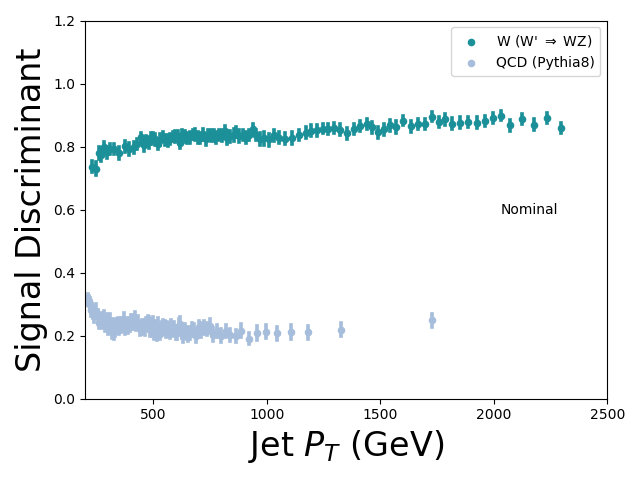
\includegraphics[width=0.4\textwidth]{figures/vtagging/lola/wLola_v6_Weighted_withM_withPT-profile-jpt.png}
\caption{The LoLa discriminant as a function of jet \PT after training with a weight intended to flatten the sample \PT spectrum.}
\label{fig:lola:ptweightedcorr}
\end{figure}
For completeness, Figure~\ref{fig:lola:nsubjcorr} shows the \nsubj and \ddt discriminants versus jet \PT. Whereas the nominal LoLa discriminant had a much larger correlation with jet \PT than the \nsubj-based taggers, the \PT-reweighted version is as decorrelated from \PT as the \nsubj variables while still exhibiting a better absolute performance than the baseline taggers.
\begin{figure}[h!]
\centering
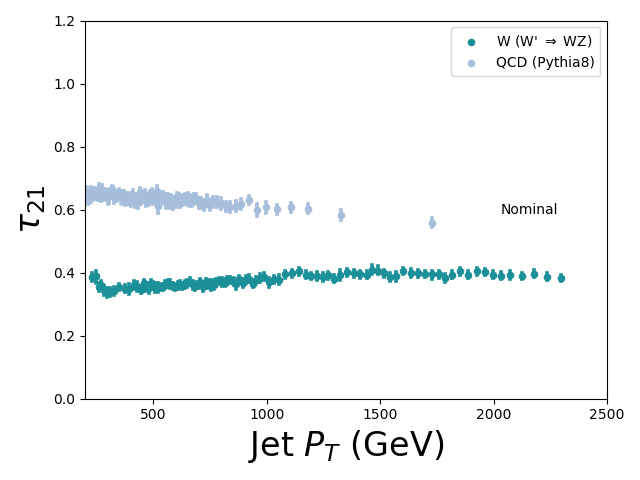
\includegraphics[width=0.4\textwidth]{figures/vtagging/lola/tau21_-profile-jpt.png}
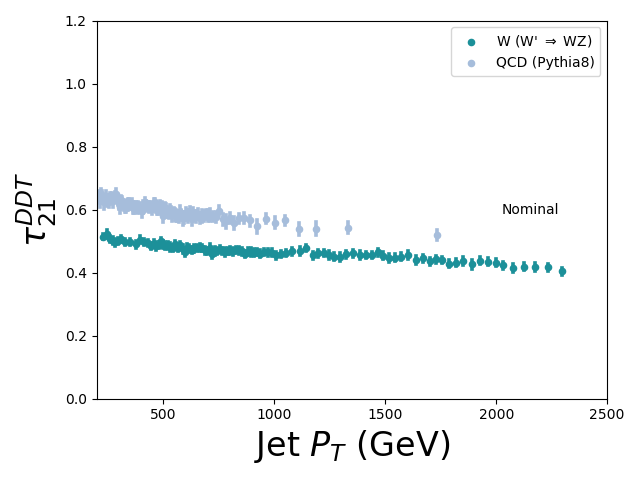
\includegraphics[width=0.4\textwidth]{figures/vtagging/lola/ddt_-profile-jpt.png}
\caption{The \nsubj (left) and \ddt (right) discriminant as a function of jet \PT.}
\label{fig:lola:nsubjcorr}
\end{figure}
In summary, reweighting strategies as the one described above yield a loss in overall performance, as expected when removing information from the training. However, the \PT dependence of the tagger is strongly reduced, meaning that it might perform better overall in physics analysis when systematic uncertainties are taken into account. There is therefore no clear answer as to which method is better before running a full analysis including systematics for \PT-dependent tagging.
 
\subsection{Mass sculpting}
\label{sec:lola:massculpting}
Any smart deep neural network intended to separate Ws from quarks and gluons, will inevitably learn the W mass as it clearly is very different from the q/g mass. Unfortunately, as these taggers are meant to be used in physics analysis where we often estimate the background in mass sidebands, this has some undesired side effects. If a deep neural network has learned the mass then, after applying a cut on the discriminant, the background jet mass distribution becomes severely sculpted and difficult to constrain. \newline
After applying a cut on the LoLa discriminant corresponding to a 1\% mistagging rate, we see in the left plot in Figure~\ref{fig:lola:masssculpt} that the W jet signal shape is nicely retained. In addition, there are no QCD jets left at low mass so no jet mass window is needed when using this tagger, leading to a significantly higher signal acceptance. However, when looking more closely at 
the QCD background on the right plot of Figure~\ref{fig:lola:masssculpt}, where all histograms are normalized to unit area, we see that the bulk of the remaining 1\% QCD jets is right below the W mass peak and has been sculpted to look exactly like the signal.
\begin{figure}[h!]
\centering
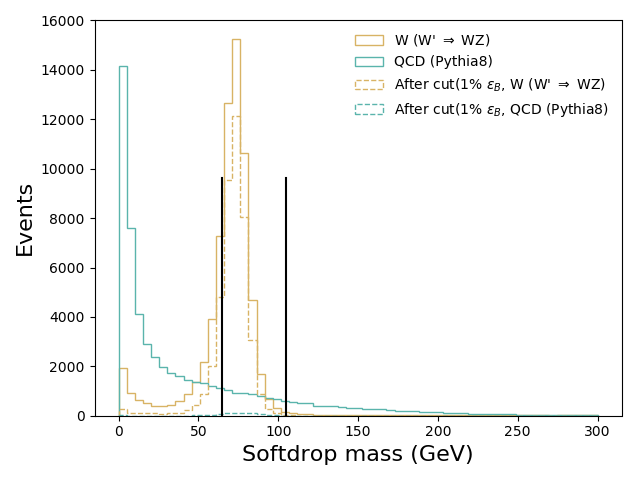
\includegraphics[width=0.4\textwidth]{figures/vtagging/lola/wLola_v6_500rew-mass-afterCut-sigprob_wLola_v6_500rew.png}
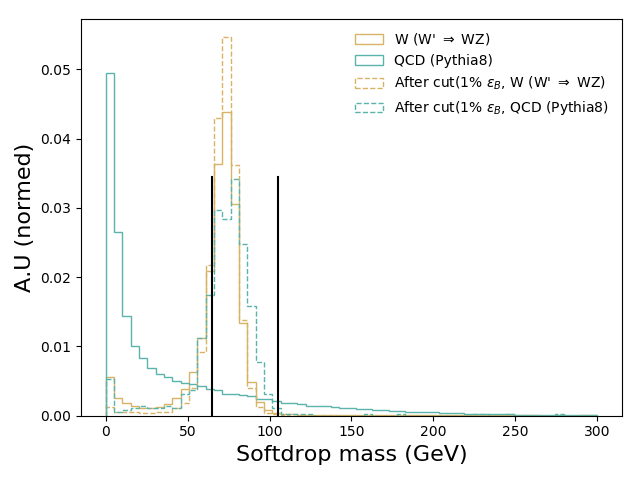
\includegraphics[width=0.4\textwidth]{figures/vtagging/lola/wLola_v6_500rew-mass-afterCut-sigprob_wLola_v6_500rew_normed.png}
\caption{The softdrop jet mass distribution before (solid lines) and after (dotted lines) a cut on the LoLa discriminant corresponding to a 1\% mistagging rate has been applied. The left plot shows the real number of events left after the cut, the right is normalized to area.}
\label{fig:lola:masssculpt}
\end{figure}
This mass sculpting is in and on its own not a problem, the tagger still manages to get rid of most of the background. However, in many physics analysis, in order to evaluate the background rate in the data signal region, mass sidebands are used. If the background distribution is peaky rather than smoothly falling, the shape and consequently the expected yield is very difficult to constrain. That leads to large uncertainties on the background rate and might eventually make an analysis less sensitive than when using a tagger with a worse absolute performance, but reduced mass correlation. In addition, if one were to search for peaks in the softdrop jet mass, as is the case for the multidimensional fit, this becomes increasingly difficult when attempting to fit a potential signal peak on top of a peaking background.\newline
It should again be mentioned, that also for the baseline taggers based on \nsubj, mass sculpting is a known feature. Figure~\ref{fig:lola:masssculpttau} shown the same softdrop jet mass spectrum before and after a cut corresponding to a 1\% mistagging rate on \nsubj (left) and \ddt (right). Here \nsubj clearly exhibits mass sculpting, but not as peaky as was the case for LoLa. \ddt exhibits the least amount of sculpting, but is also the tagger with the worst absolute performance.\par 
\begin{figure}[h!]
\centering
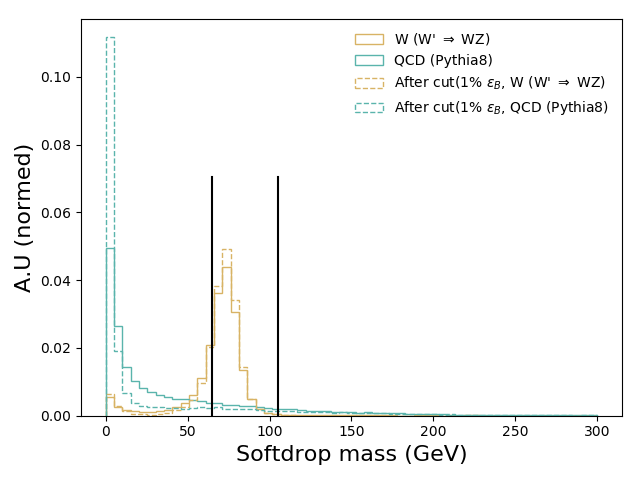
\includegraphics[width=0.4\textwidth]{figures/vtagging/lola/wLola_v6_500rew-mass-afterCut-ddt_normed.png}
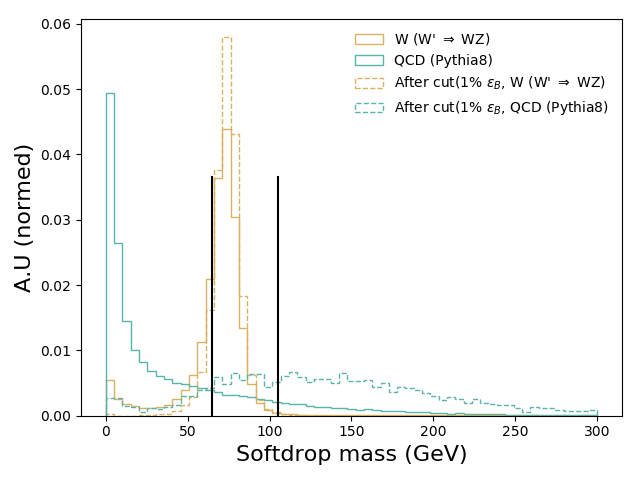
\includegraphics[width=0.4\textwidth]{figures/vtagging/lola/wLola_v6_500rew-mass-afterCut-jtau21_normed.png}
\caption{The softdrop jet mass distribution before (solid lines) and after (dotted lines) a cut on \nsubj (left) and \ddt (right). All spectra are normalized to unit area.}
\label{fig:lola:masssculpttau}
\end{figure}

I have not yet had the chance to implement a mass decorrelation strategy for LoLa, but I see two ways going forward: The first is, following the example of what was done to decorrelate LoLa from jet \PT, to pass a mass dependent sample weight to the training. LoLa would then be trained with a weight derived to flatten the two dimensional jet mass - jet \PT plane. Another option would be to train LoLa together with an adversarial, a dedicated deep neural network running in parallel to LoLa and attempting to learn the jet mass from the LoLa output. The total loss function would then be a sum of the two, where the better the adversarial is in learning the mass, the worse the total loss function gets. Both these options are something I'd like to explore in the future.\par

In summary, mass- and \PT-dependence are in their own right not a problem for a tagger. The problem occurs when using these taggers in actual physics analyses where background rate uncertainties and tagging \PT dependence uncertainties has a large impact on the final sensitivity. There is a trade-off between signal efficiency and (analysis-dependent) systematics. For LoLa, rather than choosing, I'd like to provide to different taggers: A nominal tagger, where no mass/\PT-decorrelation is attempted, and a decorrelated version. Then both can be tested in a full analysis chain before deciding on which tagger to use when looking at data.

\section{Validation on an independent sample}
\label{sec:validation}
LoLa is additionally validated on independent samples as an unbiased measure of performance allowing to compare different CMS W-tagging algorithms to one another: A $\PZpr \rightarrow WW$ sample with $M_{\PZpr}=3\TeV$ produced with MadGraph and a QCD \PYTHIA8 sample in a \PT bin of 1000 to 1400 \GeV. Here, only jets with $ 1000 \GeV < \PT < 1400 \GeV$ and $|\eta| < 1.5$ are used. The signal efficiency versus mistagging rate for LoLa compared to the baseline PUPPI Softdrop + \nsubj tagger, is shown in Figure~\ref{roc_val}. As was pointed out in Section~\ref{sec:training}, a mass cut is not necessary when using LoLa, but has been added to this plot for completeness. A significant improvement in tagging efficiency is observed for LoLa compared to the default tagger, also when being validated on a sample completely independent from the training sample. The cut corresponding to a 30 \% signal efficiency working point are used as reference working points when we will look at the tagging performance as a function of jet \PT and pileup in the following, and is marked by triangles in the plot.
\begin{figure}[h!]
\centering
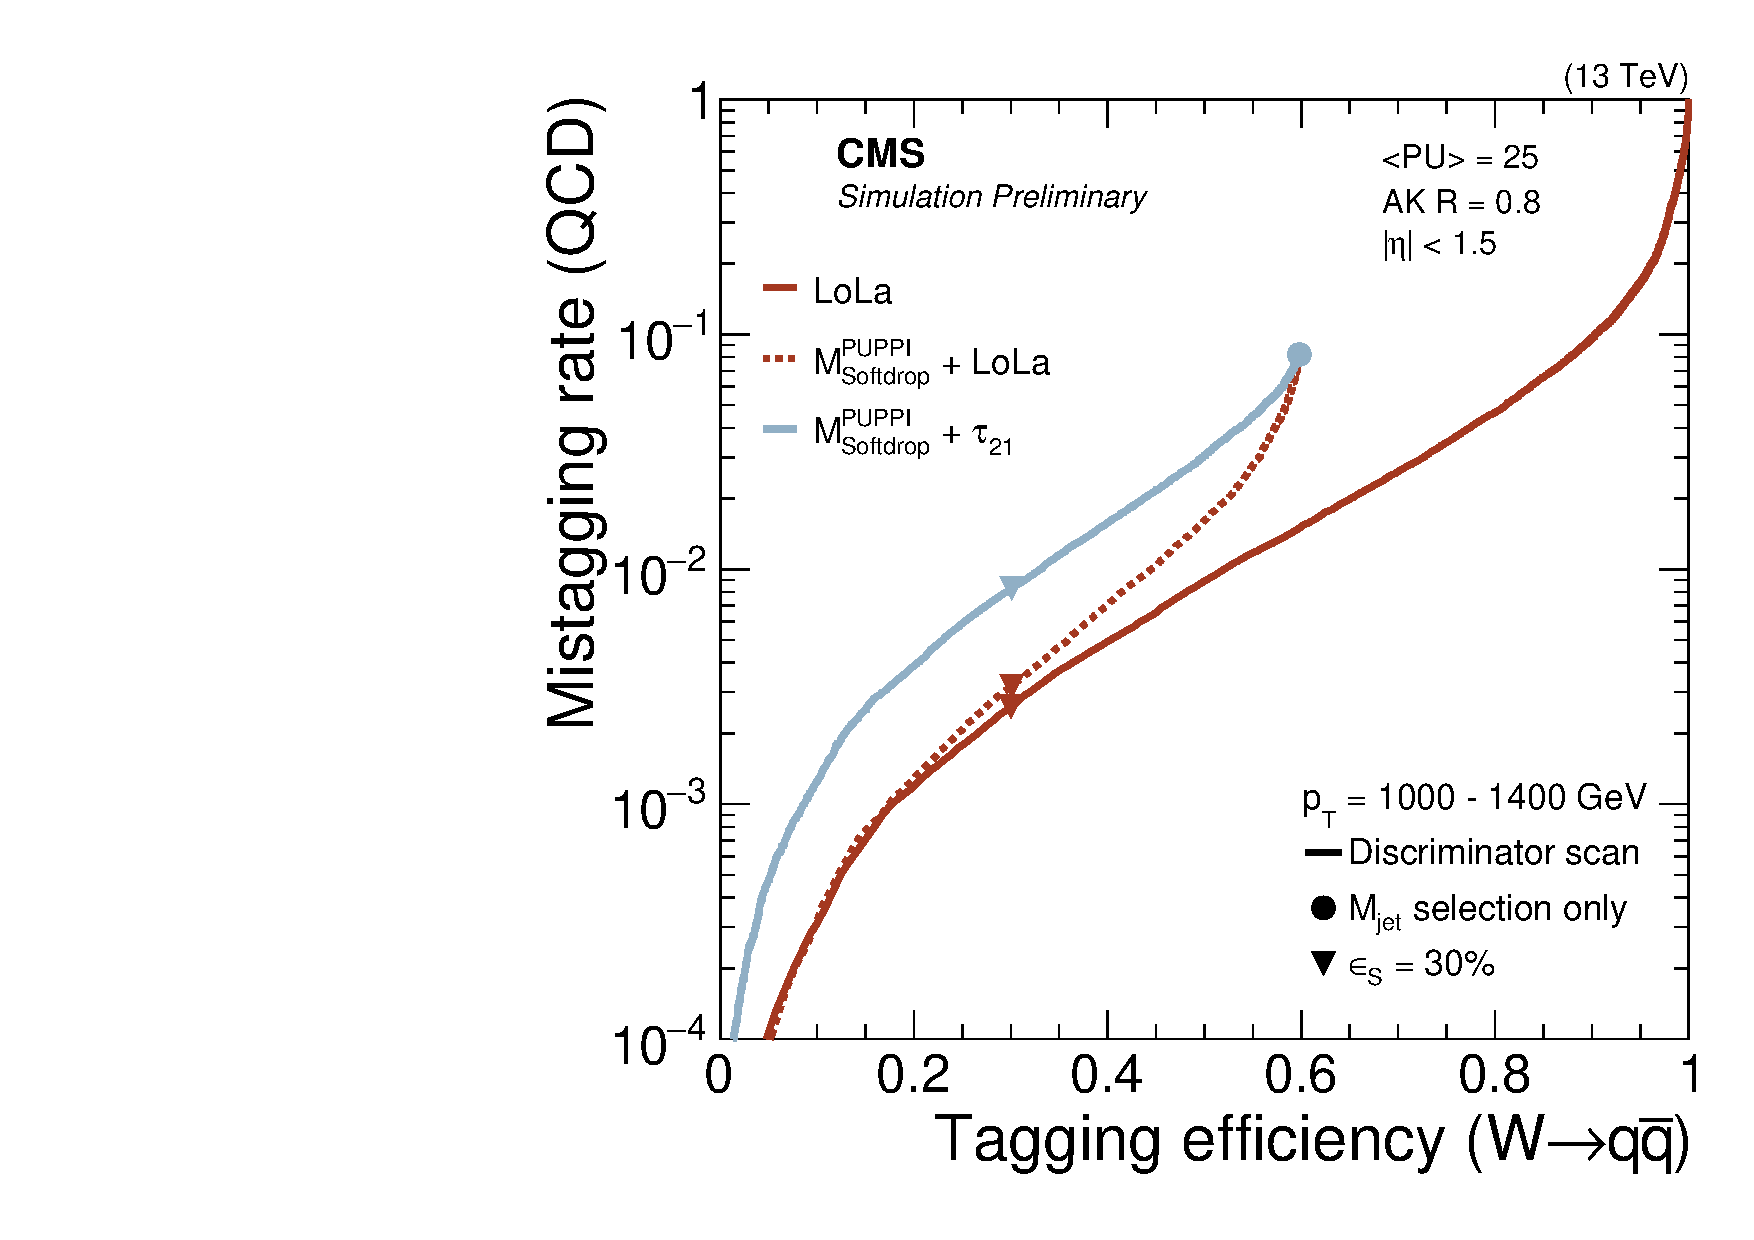
\includegraphics[width=0.4\textwidth]{figures/vtagging/AN-18-099/validation/roc_ZpWqqvsQCD.pdf}\\
\caption{Performance of LoLa and PUPPI Softdrop + $\tau_{21}$ in the background-signal efficiency plane. The PUPPI softdrop jet mass
selection of $65 < M_{SD} < 105 GeV$, and the 30 percent efficiency points are indicated with symbols.}
\label{fig:roc_val}
\end{figure}
The signal efficiency and mistagging rate as a function of jet \PT, is shown in Figure~\ref{fig:lola:eff_val_pt}. Again we observe the strong correlation between LoLa tagging efficiency and jet transverse momenta. There is, however, no point in the spectra where the \nsubj tagger has a higher signal over background ratio than LoLa. LoLa performs its worst at very high jet \PT, but in this region the background is very small (dijet invariant masses around 2.5-3 \TeV) so the absolute performance here matters less than at lower \PT
\begin{figure}[h!]
\centering
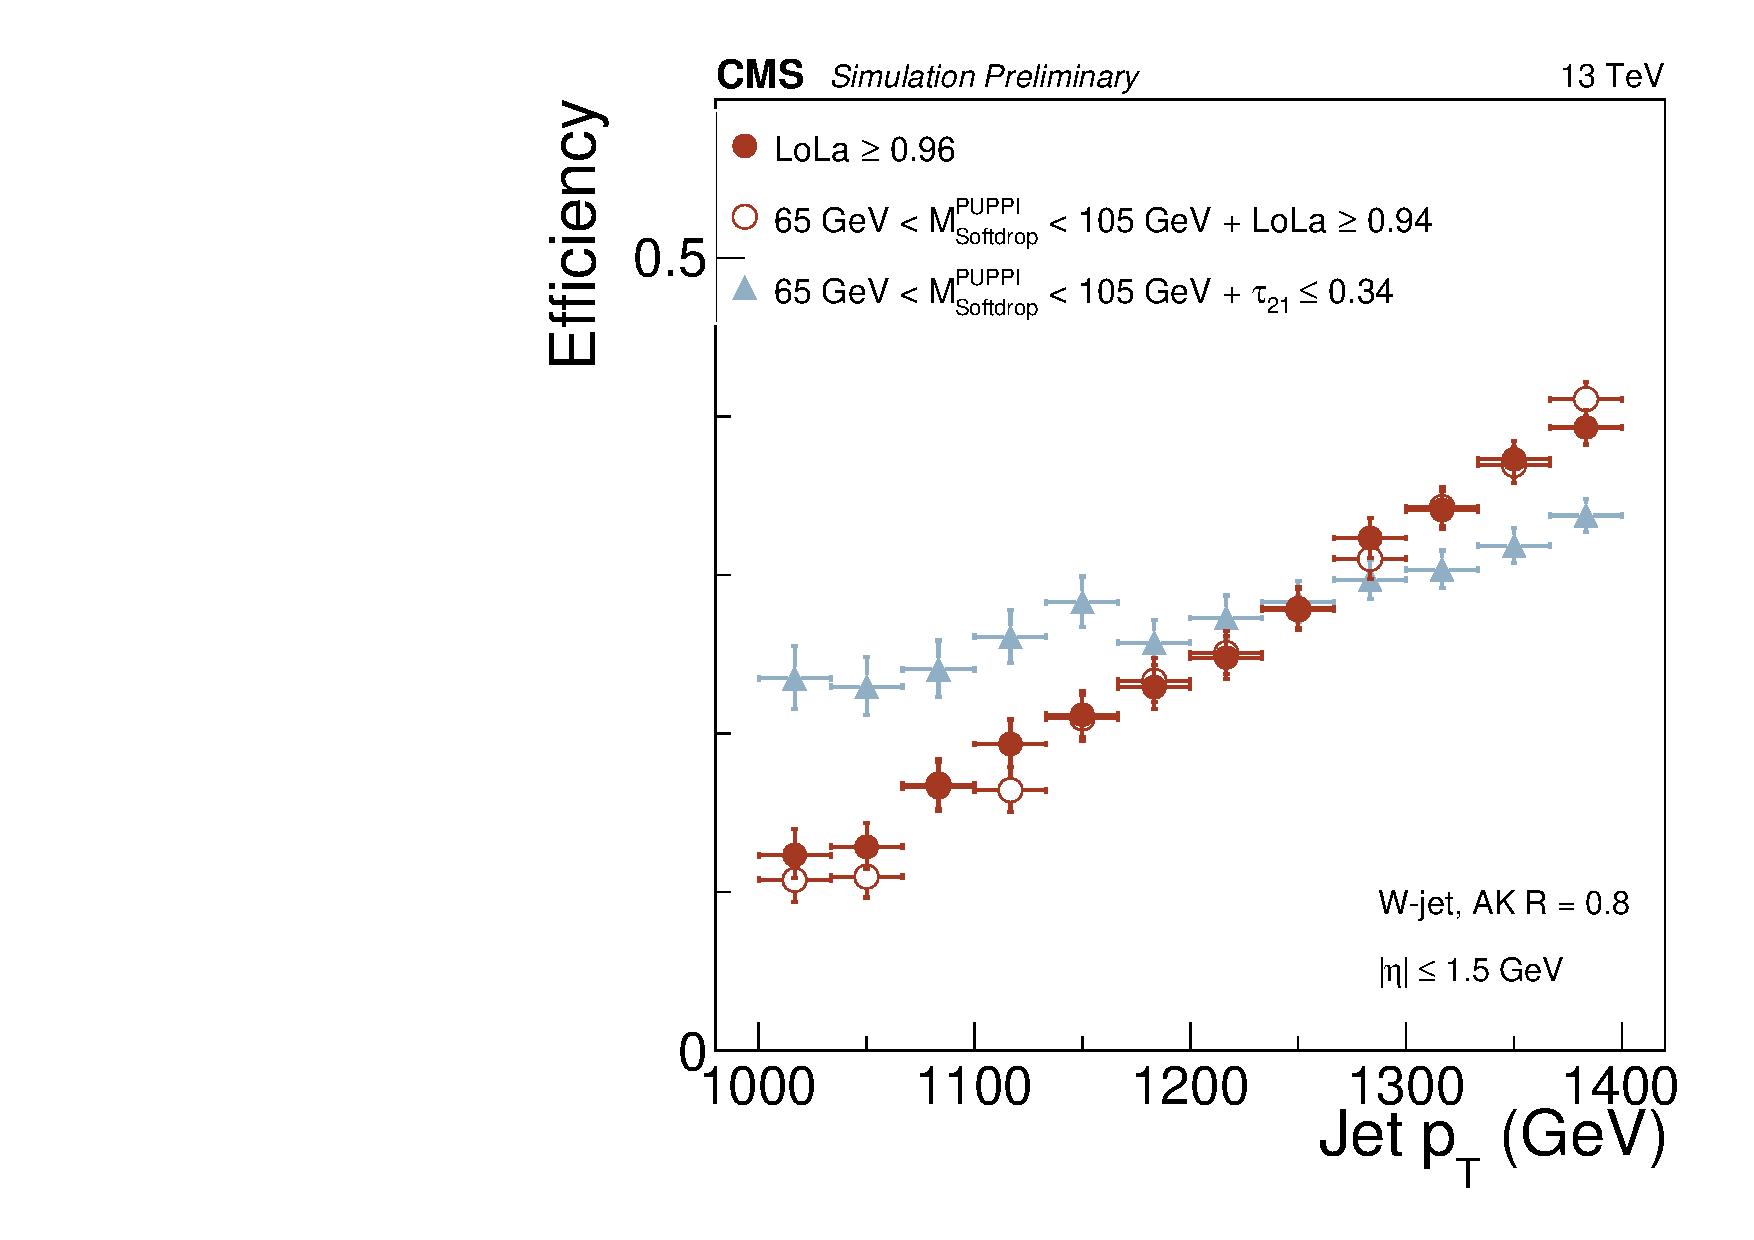
\includegraphics[width=0.4\textwidth]{figures/vtagging/AN-18-099/validation/WtagSigEffvsjpt.pdf}
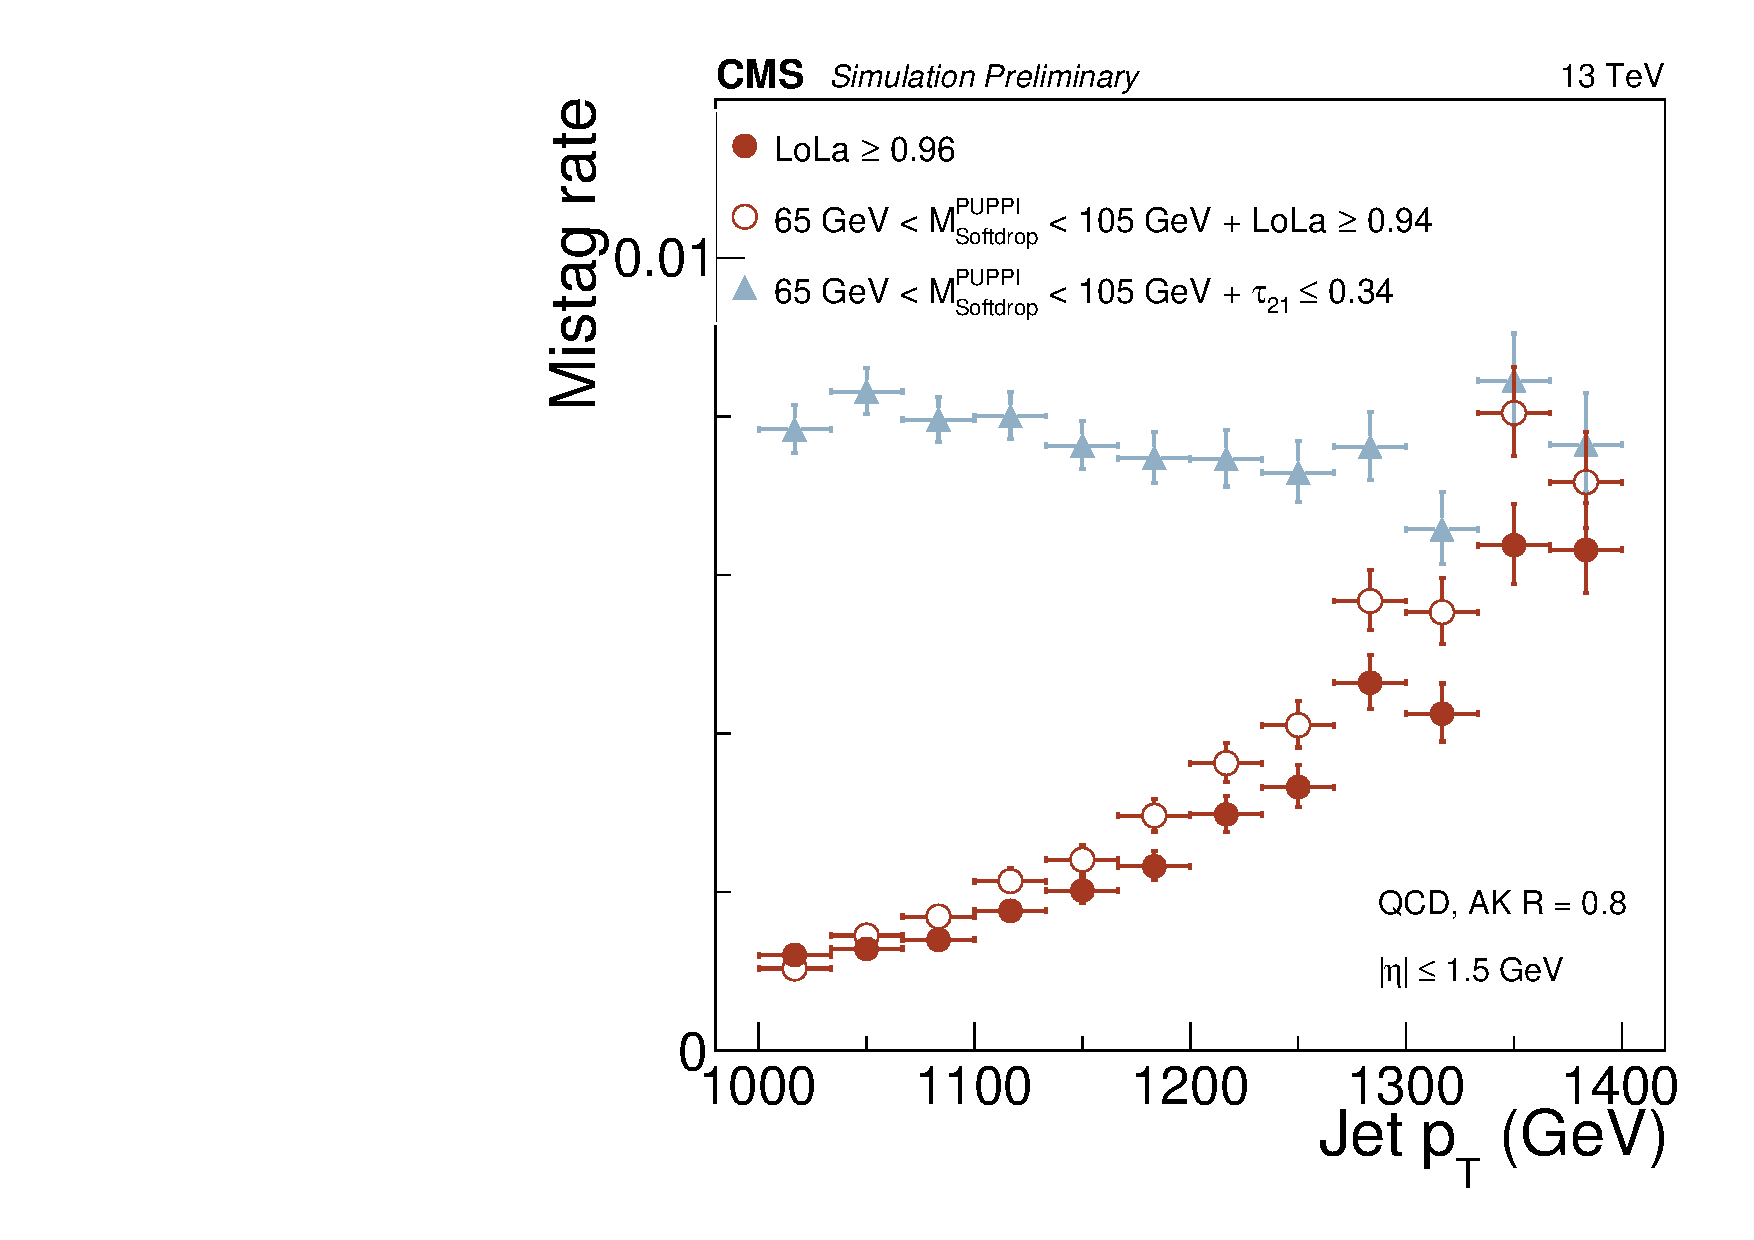
\includegraphics[width=0.4\textwidth]{figures/vtagging/AN-18-099/validation/QCDMistagvsjpt.pdf}
\caption{Efficiency (left) and mistagging rate (right) of the LoLa selection corresponding to a 30 percent signal efficiency as a function of jet \PT.}
\label{fig:lola:eff_val_pt}
\end{figure}
Figure~\ref{fig:lola:eff_val_pu} shows the tagging efficiency and mistagging rate as a function of pileup. Both taggers under study are more or less decorrelated from pileup, with a flat efficiency up to 50 reconstructed primary vertices. In Run 3, this number is of course expected to be significantly higher, around 140-200, and the study should be redone up to a higher number of reconstructed primary vertices.
\begin{figure}[h!]
\centering
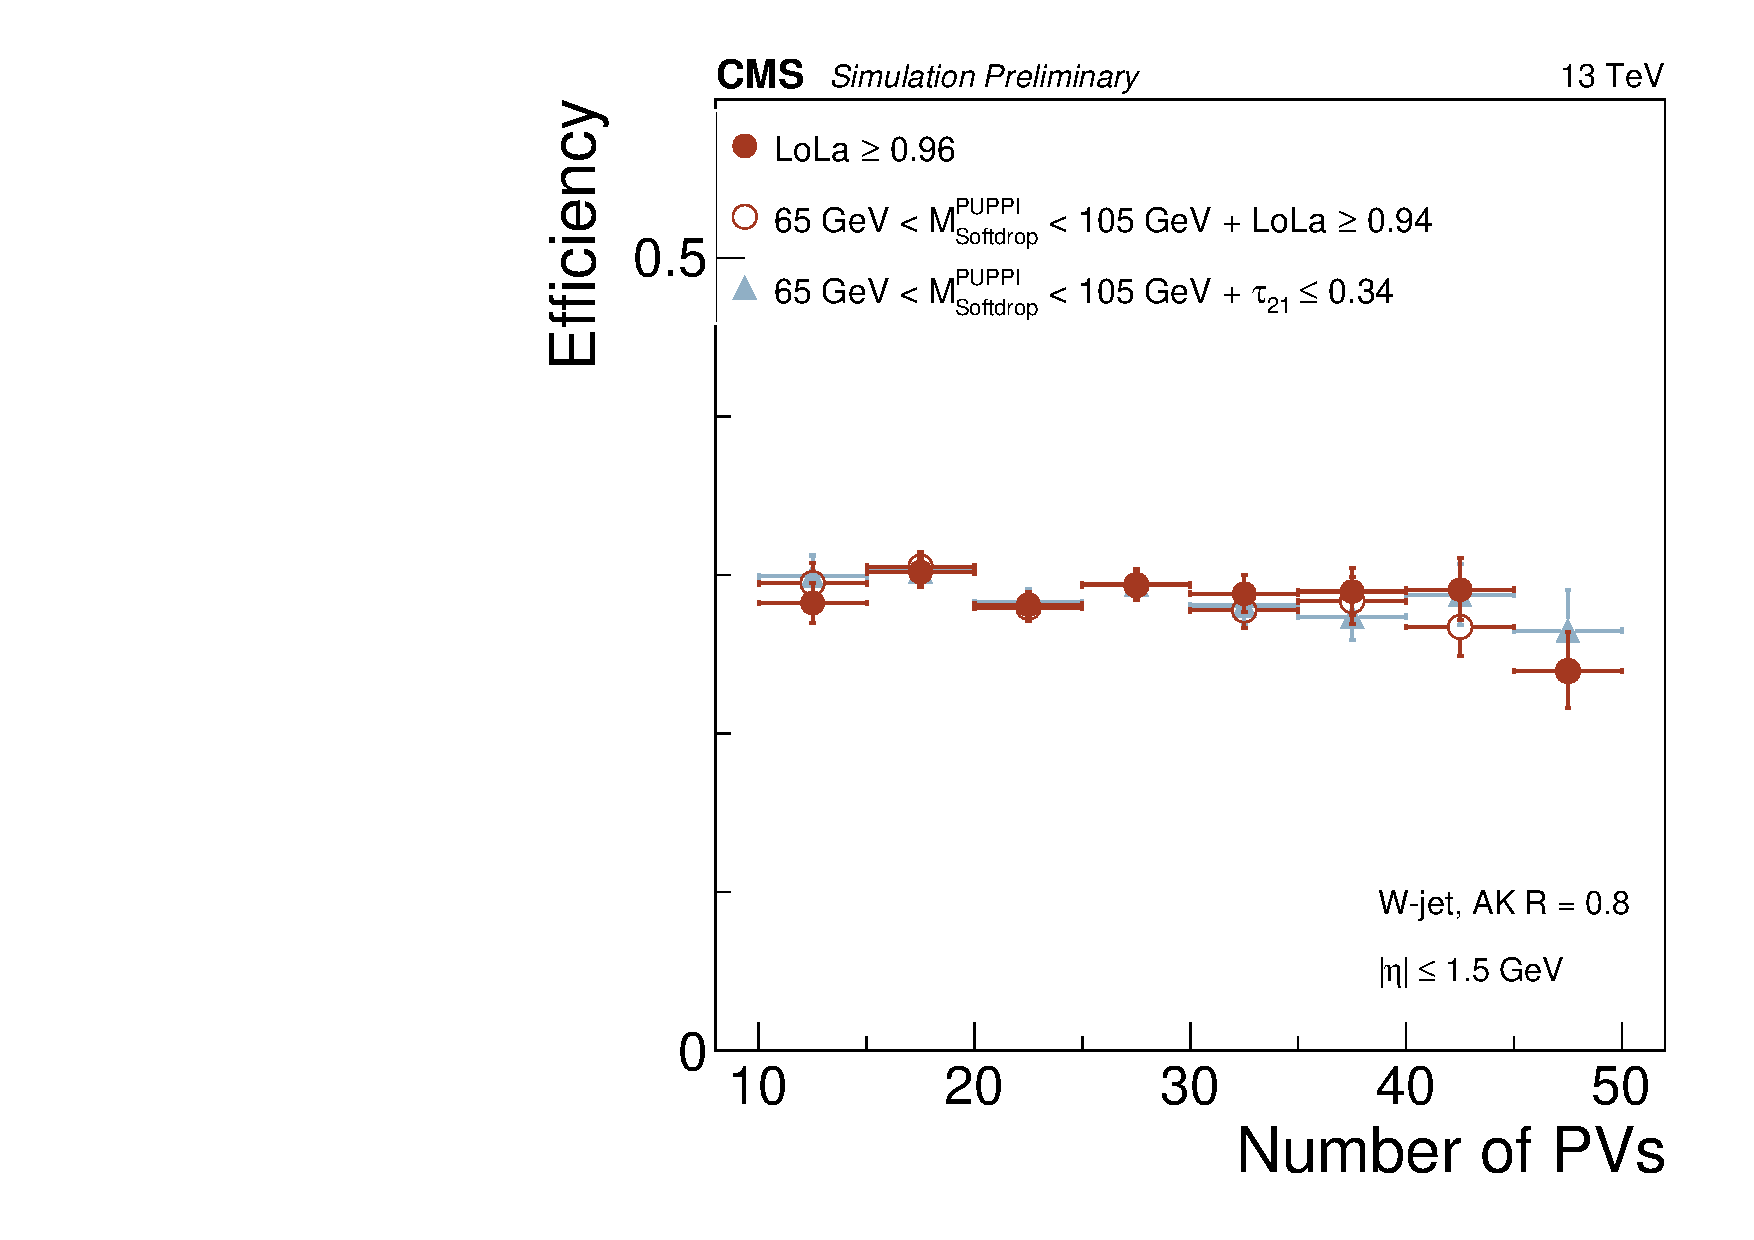
\includegraphics[width=0.4\textwidth]{figures/vtagging/AN-18-099/validation/WtagSigEffvsnPV.pdf}
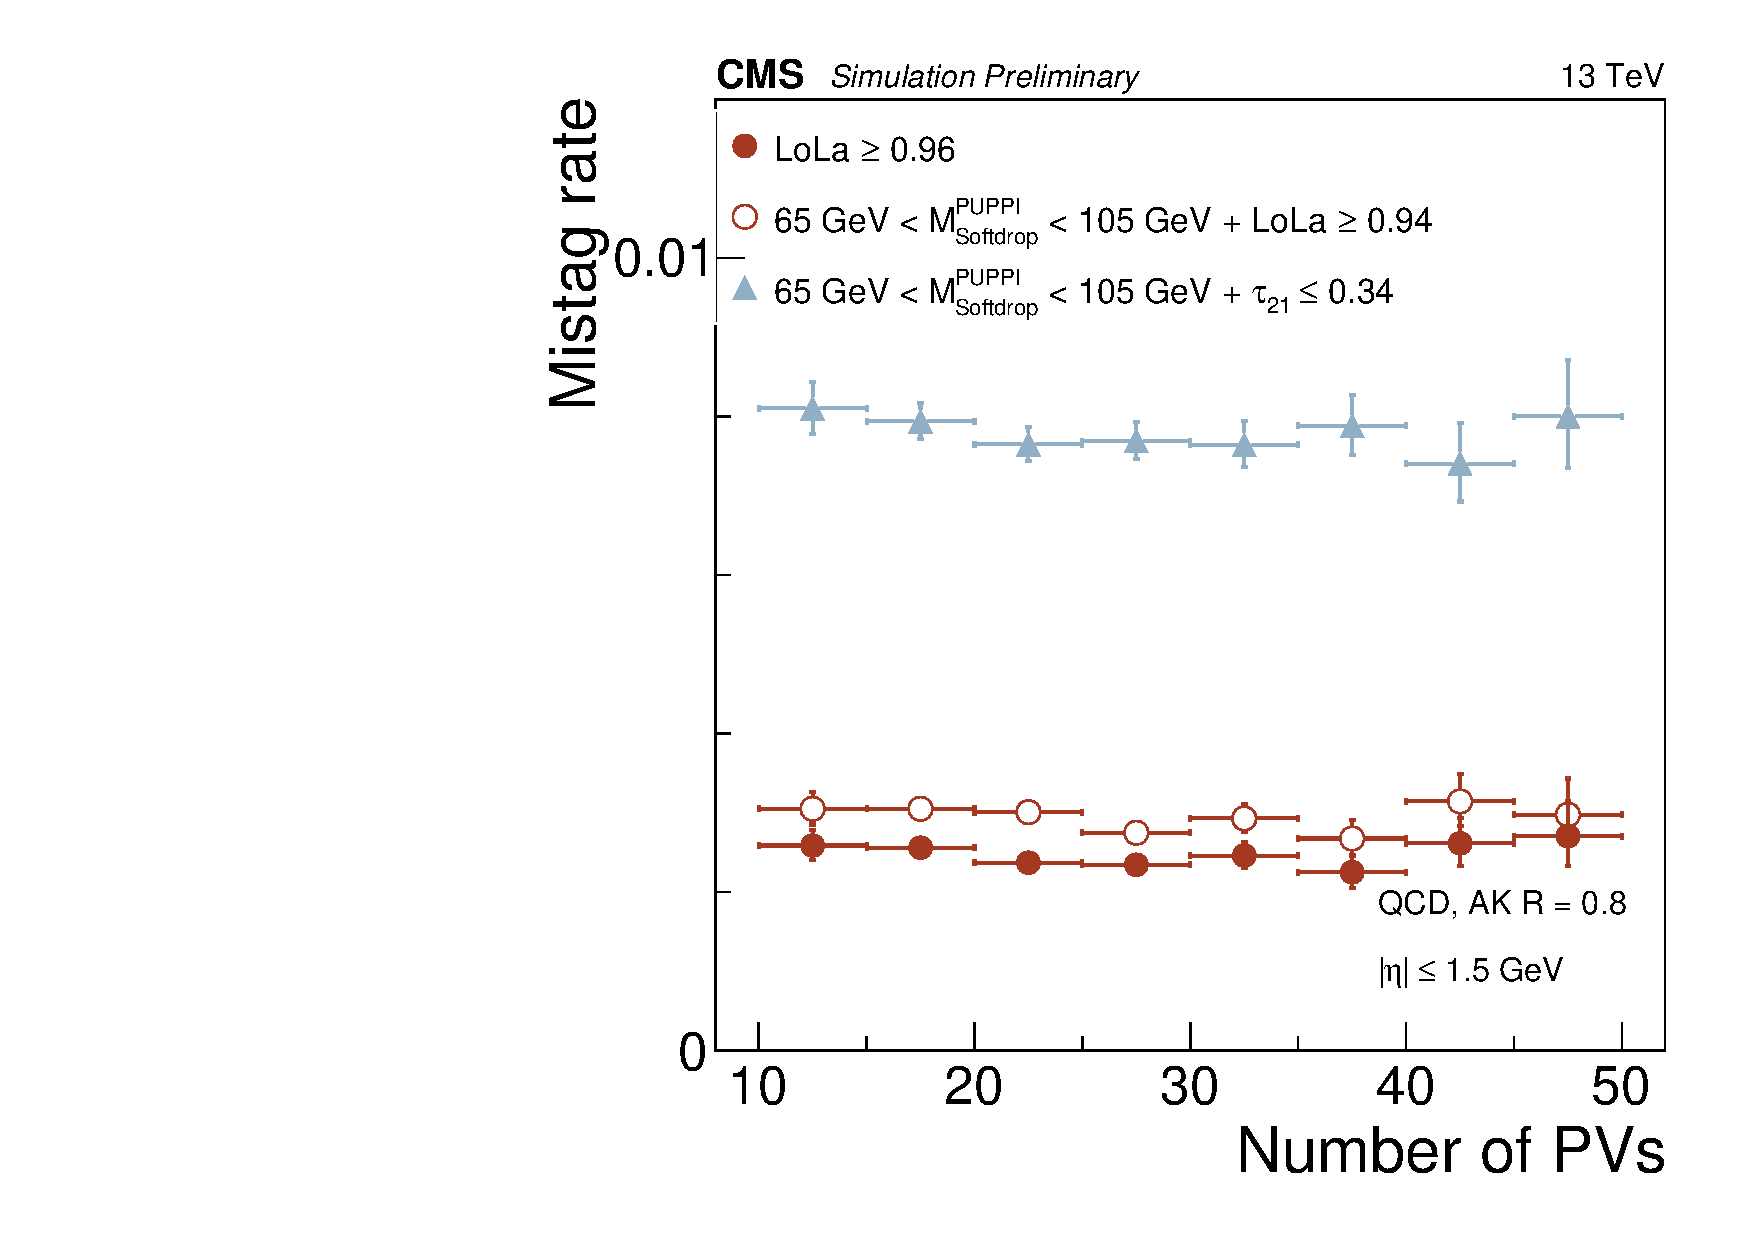
\includegraphics[width=0.4\textwidth]{figures/vtagging/AN-18-099/validation/QCDMistagvsnPV.pdf}
\caption{Efficiency (left) and mistagging rate (right) of the LoLa selection corresponding to a 30 percent signal efficiency as a function of the number of reconstructed vertices.}
\label{fig:lola:eff_val_pu}
\end{figure}
\clearpage
\section{Summary and outlook}
\label{sec:lola:outlook}
In this chapter, we have seen a promising new W-tagging algorithm for future VV searches. Its absolute performance is better than that of the baseline PUPPI softdrop + \nsubj tagger up to a jet \PT of at least 1400 \GeV, roughly corresponding to a dijet invariant mass of 2.5-3 \TeV, and could lead to an increase in total signal efficiency from 18 to 43 \% for the searches presented here. With a \PT decorrelation method already in place, it could already now be used for the one dimensional VV search presented in Search I and Search II. However, if to be used in the multidimensional search framework, a mass decorrelation method needs to be established. I have already outlined two possibilities of how to achieve this in Section~\ref{sec:lola:massculpting}, where one of these has already been shown to work in the context of \PT decorrelation. This is, as of this writing, left to future studies.
\newline
\newline
When discussing the future of the multidimensional search, I mentioned how a deep neural network such as the one presented here could be used to encode jet substructure in a way useful in order to develop a generic anti-QCD tagger. This has already been achieved by a parallel analysis team through the use of auto-encoders, published ten days before this writing and documented in~\cite{Heimel:2018mkt}, and has shown very promising results. However, this strategy is, to my knowledge after discussing with the authors, no longer pursued after observing that the auto-encoder version of LoLa was very difficult to decorrelate from the jet mass. It is my belief that this can be overcome by changing some of the features calculated in the Lorentz Layer (in~\cite{Heimel:2018mkt}, only the invariant mass is calculated and the other features listed in Equation~\ref{eq:lola:lola} are stripped away) and this is something I would also like to pursue in future studies in order to achieve the truly generic search for boosted dijet resonances in the \MJO-\MJT-\MVV plane.